
\subsection{Answers}
\begin{table}[htb]%
\begin{center}%
\caption{Q6: How long have you been writing MPI programs?}%
\label{tab:Q6-ans}%
\begin{tabular}{l|l|r}%
\hline%
Choice & Abbrv. & \# Answers \\%
\hline%
more than 10 years & \verb!>!10 & 298 (35.4\%) \\%
between 5 and 10 years & 5-10 & 202 (24.0\%) \\%
between 2 and 5 years & 2-5 & 195 (23.2\%) \\%
less than 2 years & \verb!<!2 & 147 (17.5\%) \\%
\hline%
\multicolumn{2}{c}{total} & 842 \\%
\hline%
\end{tabular}%
\end{center}%
\end{table}%


Respondents with over 5 years of MPI program experience 
accounted for 60\%. In general respondents appear to be less
experienced in MPI than in general programming (cf. Q5), corroborating 
the fact  
that MPI is learned after mastering programming. By country
comparison, 
Russia has a well-balanced distribution. Beside Japan has 
few respondents under 2 years, so there may be biased in the 
response or that Japan has not been successful in 
developing new human resources who write MPI programs.


\begin{figure}[htb]
\begin{center}
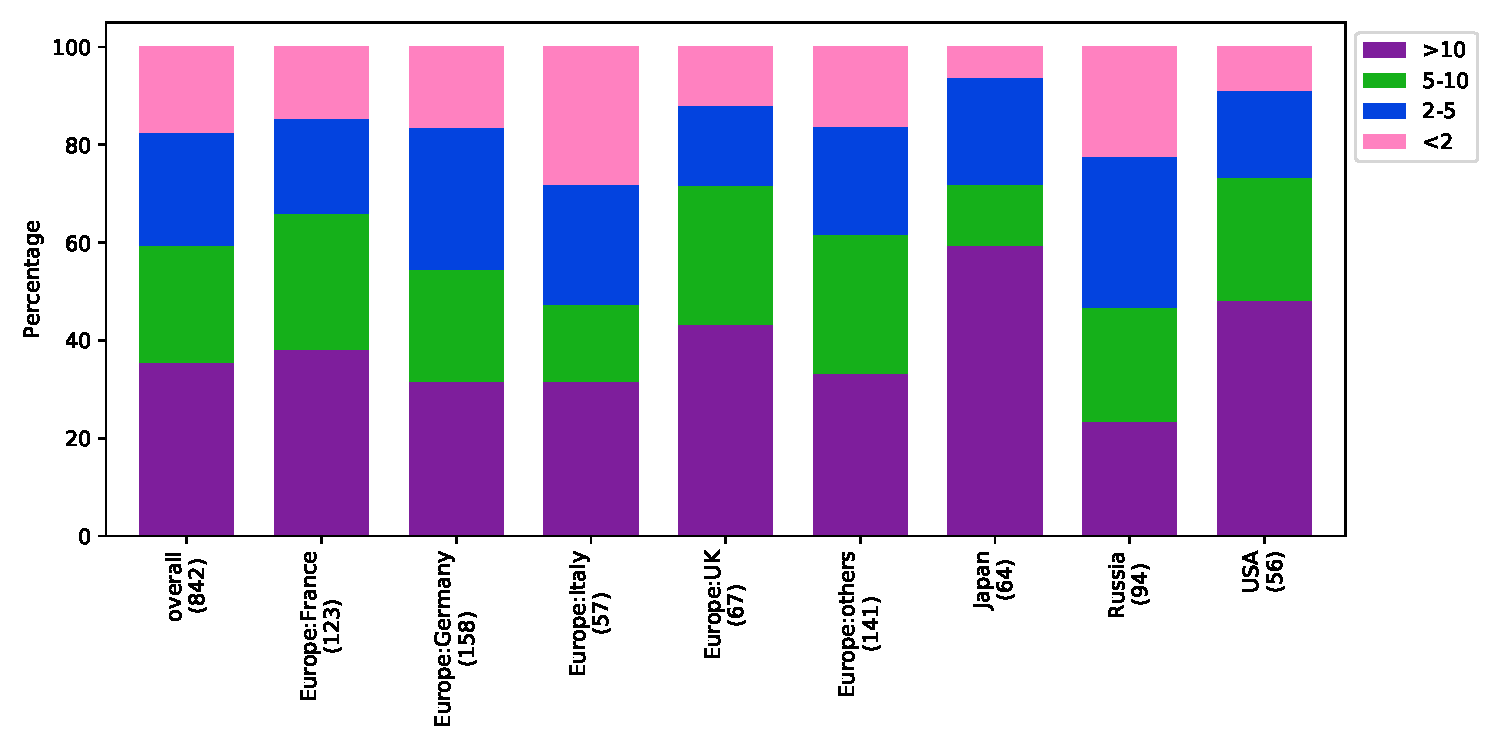
\includegraphics[width=10cm]{../pdfs/Q6.pdf}
\caption{Simple analysis: Q6}
\label{fig:Q6}
\end{center}
\end{figure}
